\documentclass[12pt,a4paper,oneside,titlepage]{article} %appel de classe
%appel des packages:
\usepackage{fontspec} %package pour gérer les fontes
\usepackage{xunicode} %package pour gérer l'unicode
\usepackage{hyperref}
\usepackage[french]{babel}
\usepackage[style=enc]{biblatex}
\usepackage{setspace}
\usepackage{csquotes}
\usepackage{graphicx} 
\usepackage{caption}
\usepackage{wrapfig}
\usepackage{parskip}


\usepackage{tikz}

\usepackage{biblatex}
\addbibresource{MASTER_ENC-Creepypasta.bib}
\usepackage{titlesec}

\author{Alexandre Lionnet-Rollin\\
	\texttt{alexandre.lionnet@chartes.psl.eu} \and \url{https://github.com/Rollybre/memoire-creepypasta}}
\title{Etude quantitative des Creepypasta : définition et caractérisation}





\setcounter{secnumdepth}{4}
\titleformat{\paragraph}
{\normalfont\normalsize\bfseries}{\theparagraph}{1em}{}
\titlespacing*{\paragraph}
{0pt}{3.25ex plus 1ex minus .2ex}{1.5ex plus .2ex}


\setstretch{1,5}
\begin{document}

\maketitle

\section*{Introduction}
	Le début des années 2000 marque l'entrée d'Internet dans la seconde phase de son existence : le Web 2.0 correspond à une période de développement sans pareils pour l'époque de nouveaux canaux de communication. L'avènement des grands réseaux sociaux tout comme les grandes plateformes d'hébergement et de partage de contenus vont permettre une nouvelle façon de dialoguer. Et parmi les nouvelles pratiques permises par ceux-ci, on trouve de nouvelles formes d'écriture, qui renouvellent aussi bien la façon d’écrire que le but des productions : écriture collaborative, écriture fragmentaire, mais aussi une écriture qui peut, à la manière d'une trainée de poudre, se répandre bien au-delà de leurs sphères de productions. Parmi celle-ci, on trouve une écriture simple, et relativement courte, prenant la forme d'un court témoignage, qui rapidement vire au cauchemar : les creepypastas. 
	

	\par
	La première occurrence du terme remonte au mois de juillet 2007 sur le forum \emph{4Chan}\footnote{Le post a depuis longtemps été supprimé. On peut néanmoins en trouver une archive au lien suivant : \url{https://web.archive.org/web/20111207000647/http://chanarchive.org/4chan/b/257/creepypasta}}. Cette dénomination est le fruit de la rencontre entre l'adjectif \emph{creepy} (litt. effrayant) et l'expression \emph{copypasta}, elle-même contraction des verbes \emph{copy} et \emph{paste} (litt. copier, coller), désignant un bloc de texte copié et collé sur différents forums afin de le partager. Si les \emph{copypastas} peuvent traiter de tous les sujets, aussi bien de blagues que de nouvelles et autres informations, les creepypastas sont quant à elles cantonnées au domaine du frisson : les creepypastas sont des copypastas dont le but est d'effrayer le lecteur. Ainsi nous nous appuierons sur cette définition de Joe Ondrak pour amorcer notre réflexion : 



\begin{quotation}
	[copypastas are] short pieces of prose, sometimes accompanied by an image or a video […] meant to be copied
			and pasted […] and spread on the Internet via social media, e-mails, and message boards […]
			whereas copypasta can be about almost any subject, creepypasta is usually aimed at scaring
			the reader and/or viewer.\footnote{\emph{Les [copypastas sont] de courts morceaux de prose, parfois accompagnés d'une image ou d'une vidéo [...] destinés à être copiés et collés [...] et diffusés sur Internet via les médias sociaux, les courriels et les tableaux d'affichage [...]Alors que le copypasta peut porter sur presque tous les sujets, le creepypasta vise généralement à effrayer le lecteur et/ou le spectateur.}}(Ondrak, 2018 p.162)\footcite{ondrak_spectres_2018}
\end{quotation}
	\par
	Cette première définition permet de souligner la dualité intrinsèque des CP : d'une part elles sont définies par leur aptitude à effrayer le lecteur (le caractère horrifique), et d'autre part par leur capacité à être transmise sur différents canaux. 
	
\section*{I.	Les caractéristiques formelles des CP}
	
\par
D’un point de vue formel, il est possible d’identifier deux caractéristiques prédominantes des CP : ce sont des productions écrites courtes et qui appuient leur narration sur la première personne. Le récit des CP prend souvent la forme d’un témoignage, d’une histoire rapportée, justifiant le rapprochement avec le folklore et les légendes urbaines\footcite{blank_slender_2018}. L’usage de la première personne est d’autant plus important car, à l’instar du folklore ou de la légende urbaine, l’histoire, et sa narration, joue avec la frontière située entre la fiction et la réalité. 
\par
La plupart des CP suivent un même schéma : un narrateur souvent intradiégétique rapporte une histoire qu’il aurait vécu. Cette histoire commence souvent de façon anodine voire trivial (vie de tous les jours, quotidien banal…), puis prend un tournant troublant voire terrifiant. 
Ce schéma n’est pas sans rappeler un autre genre littéraire: la littérature fantastique. La distance entre un personnage \emph{a priori} banal et un événement hors-du-commun est à la base aussi bien de la littérature fantastique que de l’esthétique des CP. \newline
T. Todorov, dans son \emph{Introduction à la littérature fantastique} propose comme première définition du genre  fantastique cette dichotomie: 

	\begin{quotation}
Le fantastique c’est l’hésitation éprouvée par un être qui ne connait que les lois naturelles, face à un évènement en apparence surnaturelle (Todorov, 1970, p. 27)\newline
	\end{quotation}

Cette "hésitation" se trouve aussi bien du côté du personnage que du lecteur : 
\begin{quotation}
	Le fantastique implique donc [...] l’existence d’un évènement étrange, qui provoque une hésitation chez le lecteur et le héros [...](Todorov, 1970)
\end{quotation}

Hésittation qu'on retrouve sous la forme de l'effet recherché par la CP sur le lecteur: la peur.

\par
En plus de la façon de raconter, les thèmes en eux même sont proches de ceux employés par ces genres « littéraires » : il est question de monstres sanguinaires, d’objets retrouvés, et souvent de l’enfance, le narrateur se rappelant d’évènements de sa propre jeunesse, ou faisant appel à une certaine nostalgie. Et les monstres traditionnels, s’ils sont souvent présents, laissent place dans de nombreux cas à des éléments tout aussi effrayants, mais beaucoup plus pernicieux : des éléments de notre quotidien, et particulièrement l’outil numérique. 
\par
Notons par exemple la CP \emph{Candle Cove} qui prend la forme d’une discussion sur un forum entre plusieurs utilisateurs se remémorant une émission dérangeante de leur jeunesse. Les souvenirs des uns et des autres s’ajoutent, aussi bien que les détails perturbants, jusqu’à ce qu’un utilisateur souligne le fait que sa mère s’inquiétait de le voir regarder la statique de la télévision lorsque celui-ci prétendait y voir ladite émission. 
\par
La perversion du numérique que cela soit du jeux-vidéo en passant par les vidéos et le plus souvent Internet, prolonge la remarque sur une frontière réalité/fiction friable : les objets les plus terrifiants sont souvent des objets qu’on côtoie au jour le jour sans se rendre compte de leur « potentiel horrifique ».
\par
Ainsi la mobilisation du genre de l’\emph{Analog Horror }est assez fréquente. 

Ce genre de l’horreur s’appuie sur une déformation et/ou sur la perversion de l’outil numérique dans toute sa diversité, dans le but de créer un climat dérangeant né du contraste entre l’aspect réconfortant du numérique et sa déformation\footcite{balanzategui_creepypasta_2019}. 
\par
On peut trouver une bonne illustration de ce phénomène dans les productions du type \textit{Found Footage}. Ces productions prennent la forme de vidéos, souvent déclarées comme des vidéos perdues puis retrouvées par un tiers. La vidéo réplique souvent le format VHS. Le format VHS est une norme d'enregistrement vidéo sur bande magnétique, en l'occurrence la cassette. Si la majorité des consommateurs (nous reviendrons plus tard sur ceux-ci) aujourd'hui n'ont pas connu directement l'âge d'or des VHS, celle-ci est facilement associé aux productions remontant à l'époque de leur parents, et donc potentiellement aux premières expériences de visualisation de contenu vidéo durant l'enfance, faisant ainsi du format VHS un vecteur de nostalgie.


Si les exemples sont nombreux dans le domaine du cinéma (on peut ici penser aux films \emph{The Blair Witch Project}, ou bien encore \emph{Paranormal Activity} plus récemment), on en retrouve plusieurs occurrences parmi les CP les plus iconiques : les séries de vidéos inspirées par des CP comme la série \emph{Marble Hornets} ou\emph{ The Backrooms} en sont les parfaits représentantes.

Or en plus d’un thème, le numérique fait partie intégrante de l’identité des CP. Rappelons ainsi notre définition de départ : les CP sont avant tout des productions littéraires sur Internet destinées à la diffusion sur Internet. 
	\begin{wrapfigure}{r}{5cm}
	\centering
	
\includegraphics[scale=0.35]{../../../10-19_Université_et_scolarité/17_Memoire/17.06_redaction/illustration/ben_drowned1}
	\caption{\small Un statue invoqué par le joueur: elle ne bouge pas et le suit durant sa partie, générant un malaise nouveau.}
\end{wrapfigure}

Ces objets nativement numériques ne le sont pas seulement par leur existence sur Internet mais aussi par la forme qu’ils prennent : Il n’est pas rare que les CP soient des productions multimodales, faisant intervenir d’autres médium, comme la vidéo, la photographie ou la musique. Notons par exemple la CP \emph{Ben Drowned}\footnote{\url{https://creepypasta.fandom.com/wiki/BEN_Drowned}}: classique du genre, cette CP raconte l’histoire d’un jeune homme jouant au jeu-vidéo \emph{The Legend of Zelda : Majora's Mask} acheté dans une mystérieuse brocante. \\



\emph{BEN Drowned} fait usage de tous les tropes mentionnés jusqu'ici : La narration est assurée par un narrateur intradiégétique, qui se trouve être un jeune homme, à la première personne ;  une suite d'évènements paranormaux ont lieu sans que le narrateur ou le lecteur soient en mesure d'expliquer; le jeu dont il est question est un jeu célèbre, souvent parmis les première expériences vidéoludiques de beaucoup, et donc en un sens nostalgique.
S'ajoute à cela la forme de cette CP : le récit du narrateur est entrecoupé d'extrait vidéo issu du jeu, montrant les différents bugs ou distorsion absente du jeu original.

Cette CP est emblématique car elle met en lumière la dualité fondamentale des creepypastas : puisant à la fois dans le folklore et la tradition littéraire fantastique, ainsi que dans une culture numérique, tant par ses thèmes que par sa forme assumant cette modernité numérique, les creepypastas opèrent comme un carrefour entre deux univers distincts. En s'érigeant comme récit recombinant\footcite{jacobs_character_1990} mêlant le neuf au vieux, cette convergence peut être analysée à la lumière du concept de culture de la convergence, développé par Henry Jenkins\footcite{jenkins_convergence_2006}.

Henry Jenkins a principalement exploré la convergence entre une culture industrielle traditionnelle, dominée par de grandes sociétés, et une culture numérique émergente, caractérisée par la collaboration et la participation active des individus. Toutefois, dans le contexte des creepypastas, cette hiérarchie traditionnelle n'est pas aussi pertinente. En effet, les creepypastas sont des œuvres nativement numériques, voire intrinsèquement connectées, où le rôle des médias traditionnels n'est pas aussi central. Ainsi, la dynamique de convergence se manifeste davantage à travers une analogie entre les médias et canaux traditionnels d'une part, et les grandes creepypastas qui agissent comme un canon de la culture numérique, d'autre part.

Il est essentiel de souligner la distinction du cadre théorique entre la culture de la convergence traditionnellement étudiée par Jenkins et la convergence observée dans le contexte des creepypastas. Alors que Jenkins se concentre sur la fusion entre les industries médiatiques traditionnelles et les nouvelles formes de médias numériques, l'analyse des creepypastas révèle une convergence plus subtile entre les traditions narratives anciennes et les formes d'expression contemporaines, façonnées par l'ère numérique. Ainsi, la convergence dans le domaine des creepypastas offre un exemple unique et éclairant de l'évolution des cultures narratives à l'ère numérique.



\section*{II.Les CP : du pareil au mème ?}
	
	Cette notion de parcours, de trajectoire nous permet de revenir au second élément de définition d’une CP. Nous avons mentionné jusqu’ici l’importance de la forme, du caractère terrifiant, percutant et facilement réplicable. Ce dernier élément rentre dans les faits à son tour dans une définition des CP comme une production qui est faite pour être partagé et copié. Cette définition d’un élément textuel ou plus globalement culturel qui existe dans le but d’être copié, est celle d’un même comme défini par Richard Dawkins dans les années 1970.\footcite{dawkins_gene_2003}
	\subsection*{Les CP comme mème}
	R.Dawkins définit le mème en étendant la conception du gène à un élément culturel, et non plus simplement biologique : le mème à l’instar du gène, est un réplicateur, qui ne se transmet non pas par les gamètes, mais par imitation d’un autre membre du groupe d’appartenance. Pour ce qui est d’une CP, il est difficile de ne pas la concevoir comme un mème tant sa raison d’être est d’être imité, comme l’origine du mot le laisse sous-entendre. 
	Ainsi, il convient de se demander à l’instar d’un gène, comment une CP survie dans le ‘pool de CP’(sic) pour reprendre l’expression de Dawkins ? 
	Les 3 caractéristique que souligne l’auteur sont : la longévité, la fécondité, et la fidélité de copie. Parmi ces caractéristiques, R. Dawkins exclut rapidement la première, en considérant que la question de la longévité importe peu : tant qu’une copie existe qu’importe la durée de vie d’une copie\footnote{« La longévité de n’importe quelle copie d’un mème est probablement relativement peu importante, comme c’est le cas pour n’importe quelle copie d’un gène. » \cite[voir p.218]{dawkins_gene_2003}}. Néanmoins dans notre cas, la question de la longévité est cruciale : Internet n’agit pas comme une archive sans fin. Au contraire, il est assez fréquent que des productions nativement numériques disparaissent\footnote{C'est le cas par exemple de l'\emph{ARG} \emph{This house has people in it}, jeu de piste en ligne dont la grande majorité des ressources sont aujourd'hui indisponibles}. 
	
	Dans le cas d’une CP, on peut distinguer plusieurs formes de longévité : la longévité sur la plateforme d’origine, la longévité d’une copie sur une autre plateforme ou bien encore la longévité « absolue » c’est-à-dire son espérance de vie de la première publication, en passant par toutes ses copies. Or celle-ci est difficilement quantifiable et représente en enjeu clé : remonter à l’origine d’une CP n’est pas évident, du fait de sa nature.

 Les deux autres caractéristiques sont toutes aussi importantes : est-il possible de mesurer cette fécondité ? Si la fécondité d’un mème scientifique est mesurée par son nombre de citation, est-il possible d’identifier de quoi quantifier cette fécondité pour les CP ? De même pour la fidélité, il serait intéressant de voir comment une ou plusieurs CP ont pu subir transformations et changements au cours de leur existence. Enfin, toujours dans le cadre théorique du mème, il serait intéressant de voir si la fécondité est liée à certaines caractéristiques textuelles. Autrement dit, il serait intéressant de voir s’il existe certains tropes ou façon de faire d’un point de vue littéraire qui agissent sur la survie ou réussite d’une CP.
	
	\subsubsection*{Les différentes trajectoire d'une CP}
	
	Ces 3 caractéristiques constituent une première base, mais ne représente pas une fin en soi. En effet, ces caractéristiques assez générales ne permettent pas de rendre compte de la diversité des trajectoires potentielles d’un mème et par extension d’une CP .
	
	Par définition, la CP est transmise par simple copier-coller : une fois produite sur un forum donné (par exemple \emph{4Chan}), celle-ci se retrouve copiée puis collée sur le même forum, ou dans le cas échéant sur d’autres forums. Cette forme de transmission (forme historique du genre) était particulièrement pertinente à une époque où les forums ne pouvaient archiver indéfiniment les publications (c’est le cas de \emph{4Chan}, berceau de bon nombre de CP devenue aujourd’hui incontournable, où les posts, après 24h d'inactivité, se voient supprimé) : le copier-coller était donc un moyen de survie pour les CP. 
	
	\paragraph*{Les super CP}
	
	Afin d'illustrer ce principe, prenons l'exemple d'une des CP les plus emblématiques : SCP-173\footnote{\url{http://fondationscp.wikidot.com/scp-173}}
	
	Parmi les grandes CP qui ont traversé le paysage internet, SCP-173 passe difficilement inaperçue. Apparue sur le sous-forum /x/ de \emph{4Chan}, cette CP est composée d'un court texte et d'une image. Si l'image est dérangeante, le plus important se trouve dans le corps du texte : l'entité photographiée est décrite, de telle sorte à nous laisser penser qu'un groupe, ou un organisme paragouvernemental s'en occupe, mais surtout de telle sorte à ce qu’on comprenne que cette créature n'est pas la seule retenue dans l’ombre. 

		\begin{wrapfigure}{l}{7cm}
		\centering
		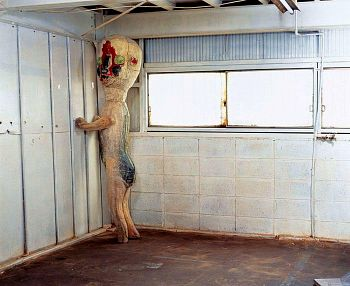
\includegraphics[scale=0.5]{../../../10-19_Université_et_scolarité/17_Memoire/17.06_redaction/illustration/SCP_173.jpg}
		
		\caption{\small \emph{Untitled 2004} créée par Izumi Kato. Cette photographie a été prise par Keisuke Yamamoto.}
	\end{wrapfigure}
	
	Durant plusieurs jours, SCP-173 s'est retrouvé copié puis collé (complétant ainsi, avec le caractère terrifiant son appellation de CP) sur le sous-forum /x/ puis sur la page d'accueil du site (le \textit{board} /b/), jusqu'à ce que d'autres utilisateurs se joignent au mouvement et produisent à leur tour d'autres CP inspirées par la forme et l'univers de cette CP originelle.
	C'est la suite de son cheminement qui fait passer cette histoire de simple CP à véritable canon : au fil des ans la communauté qui s'est construite autour de SCP-173 et de ce qu'on nomme désormais la \emph{Fondation SCP} s'est autonomisée, créant un wiki dédié (une première fois grâce au CMS \emph{EditThis} puis au CMS \emph{Wikidot}) puis continuant de croitre. Aujourd’hui la \emph{Fondation SCP} est présente dans 12 langues différentes et est forte de plusieurs milliers de productions originales dans chacune de ces langues. 
	
	Cette progression et ce rapport à une création de base peut nous amener à penser les CP comme une forme de fanfiction\footcite[voir p. 2]{goudet_agentivite_2021}.
	
	Ce rapprochement peut apparaître comme pertinent car, à l'instar d'un texte canonique source, les CP va être copié, annoté puis inévitablement modifié et ces modifications vont produire des textes à part entière. On note aussi la proximité en termes de moyen de production : l'écriture est collaborative en ce qu'elle produit une œuvre fragmentaire et asynchrone, chacun produisant à son rythme des éléments supplémentaires.
	
	De plus on trouve une dynamique similaire à celle que les fanfictions entretiennent avec le canon : l'idée de fanon\footcite{lata_du_2022} , où la production qui découle de l'œuvre originale (et donc canonique) va tirer son autorité de cette massivité\footcite{cook_canonicity_2013}. 
	Néanmoins cette analogie ne fonctionne que dans de rares cas. Les CP sont majoritairement des textes uniques, d'effrayantes bouteilles jetées à la mer par un utilisateur, qui n'a pas vocation à s'établir comme récit fondateur. 
	
	SCP-173 est donc un des rares exemple de cette trajectoire particulière : celle d'une CP prenant tellement d'ampleur qu'elle devient elle même la base d'un canon ou d'un \textit{fandom}. 

	
	Il n'existe que trois exemples de cette trajectoire : SCP-173 et la \emph{Fondation SCP}, les \emph{Backrooms} et \emph{Slenderman}. 
	Ces trois cas suivent une trajectoire similaire: une première publication sur un forum (respectivement \emph{4Chan} et \emph{SomethingAwful}), une vague importante de réaction sur ce même forum, puis une "exportation" vers une plateforme dédiée. Si la trajectoire globale est la même, chacune de ces CP a des caractéristiques formelles et "trajectorielle" propre (changement de forme et/ou de média).
	
	\paragraph*{Les CP historiques}
	
	Alors que toutes les CP ne suivent pas la même trajectoire qui restent largement exceptionnelles, certaines productions, dès les débuts de ce genre, ont laissé une empreinte indélébile sur le lectorat. Elles se sont hissées au rang de références, d'histoires marquantes qui ont contribué à définir le genre. 
	
	Ces CP, que nous qualifierons de CP \textbf{historique}, ont suivi un début de trajectoire similaire, mais ne se sont pas hissées au rang de canon. Malgré cela elles ont connus un franc succès. Ce succès ne prend pas la forme d'histoires liées mais par des reproductions sur d'autres formes. Au delà d'un simple copier-coller, ces histoires ont été narré sur d'autres plateformes,ou bien illustré sous différentes formes (animations, dessin...). 
	\textit{Ben Drowned}, que nous avons mentionné plus tôt, est un exemple de cette trajectoire : en plus de sa navigation sur différents forums, de nombreux utilisateurs, sur Youtube par exemple, utilise les images du jeux présentes dans la CP originale pour illustrer tout en narrant l'histoire associée\footnote{Voir par exemple \url{https://www.youtube.com/watch?v=2o7lcKHjdoQ\&pp=ygULYmVuIGRyb3duZWQ\%3D}}, ou ont cherché à expliquer, approfondir l'expérience\footnote{\url{https://www.youtube.com/watch?v=QJlqY1O4B00}}.
	On peut citer, à titre d'exemple, les CP \emph{le syndrome de Lavanville} \footnote{\url{https://creepypasta.fandom.com/wiki/Lavender_Town_Syndrome}} qui évoque une rumeur sur la musique d'une version d'un jeu Pokémon, ou encore \emph{Squidward's Suicide} \footnote{\url{https://creepypasta.fandom.com/wiki/Squidward\%27s_Suicide}}, histoire d'un épisode disparu du dessin-animé \emph{Bob l'Éponge}.

	\paragraph*{Le reste des productions}
	
	Aujourd’hui néanmoins les différentes plateformes ne sont plus assujetties à une telle limite : ce faisant le mode de production et de diffusion des CP a évolué.
	Désormais, l’écrasante majorité des CP est produite sur des forums et sites dédiés (sans que cela soit néanmoins nécessaire, comme le montre l'exemple récent des \emph{Backrooms}, apparu la première fois sur \emph{4Chan}). Les deux pôles principaux de productions de CP sont aujourd'hui le \emph{subreddit} r/nosleep \footnote{\url{https://www.reddit.com/r/nosleep/}} et le fandom Creepypasta \footnote{\url{https://creepypasta.fandom.com/}}. 
	
	Ces deux plateformes voient  quotidiennement de nouvelles histoires apparaître : ainsi si la diffusion et la viralité était un moyen de survie, les histoires produites sont désormais assujetties à des règles et des méthodes biens différentes. Ce faisant une nouvelle façon d'exister, une nouvelle trajectoire, s'est développée avec la sédimentation du "genre" au cours de ces dernières années. 
	
	Il convient néanmoins de noter dès maintenant une différence cruciale dans le fonctionnement de ces deux plateformes : en plus d'accueilir du contenu produit régulièrement le fandom Creepypasta joue aussi un rôle d'"archive" des CP historiques. 
	
	Cette sédimentation, liée à la production massive de CP \footnote{Le Fandom compte près de 14 000 pages} , entraîne aussi une attente différente vis à vis de la qualité des productions : d'un genre spontané, la CP s'est construite au fur et à mesure comme un genre travaillé. \footcite{garcia_roca_creepypasta_2021}
	

	Les plateformes accueillant ces productions ont donc développé des standards de création devant être respectés sous peine de ne pas pouvoir publier. 
	Avant de rentrer dans la description des règles de ces plateformes, l'existence même de celles-ci est intéressante : il existe désormais une attente liée à la littérarité des CP. Cette littérarité, comme nous l'avons laissé sous-entendre, n'est pas évidente : des productions anonymes sur des canaux de diffusion nouveaux et souffrant encore d'un manque de légitimité sont autant d'indice quant à un décalage entre les productions littéraires patrimoniales et les productions numériques.
	
	La question de la littérarité ("c'est-à-dire ce qui fait d'une œuvre donnée une œuvre littéraire" ) est, d'un point de vue quantitatif (et donc du point de vue de la forme et non du fond), définissable sous différentes formes: le but est de mettre en avant une complexité textuelle caractéristique des œuvres littéraires, des caractéristiques qui différencieraient les textes de simple publication sur un forum.

	La première hypothèse qu'il est possible d'émettre tiens à la sédimentation du genre : avec l'apparition d'attentes liées à la qualité, on peut conjecturer l'apparition ou la croissance de la littérarité des textes avec le temps.
	%Il y a mélange entre qualité et longévité : une CP qui reste dans le temps (enfin qui existe) est une CP qui respecte des règles .

	Ainsi une première étape dans la perspective d'une analyse génétique se dessine : peut on voir se dessiner des tendances dans la littérarité des production littéraires ? 


	Pour ce faire, il est possible de mobiliser et de comparer des métriques comme la longueur des texte, la taille des phrases, la complexité du vocabulaire ou des indices lisibilité (\textit{readability}). 
	En plus de l'étude de l'évolution dans le temps, il peut être intéressant de déterminer si ces différents indices de littérarité évoluent ou sont présents/absents de la même manière sur les différentes plateformes : cette analyse permettra de dresser la présence ou l'absence de similarité dans la forme au sein des différentes plateformes, et donc de déterminer une forme d'autorité propre à chaque plateforme.\footcite{mayer_autorite_2017}
	
	
	\section*{Récupération des données}
	
	La récupération des données a nécéssité une méthode différente pour chacune des plateformes.  En effet, le moissonnage des données présentes sur le web est dépendant à la fois de la forme de la plateforme et des données qui y sont présentes tout comme de la potentielle politique d'utilisation et de récupération de celle-ci. 
	
	Pour ce qui est du fandom CP, la récupération des données a été relativement facile : le site n'est pas structuré sous la forme d'un arbre, comem on pourrait s'y attendre. Au contraire, une grande partie du site, dont les histoires à récupérer font parties, n'est pas hiérérchisé. Ce faisant, il n'est pas possible d'utiliser l'organisation du site pour repérer et récupérer les différentes publications.
	Cette structure ne permet pas une méthode "brutale" qui consisterait à récupérer l'ensemble du site puis filtrer les pages qui nous intéressent en fonction du lien.
	
	A défaut de hiérarchisation, le site utilise une structure par hyperlien. Ainsi pour accéder à une partie du site il faut : la chercher explicitement,ou dans la plupart des cas, y accéder en appuyant sur un lien présent sur un page. 
	Ainsi, afin de récupérer les publications, il est nécessaire de trouver une page qui renverrait vers toutes les autres publications. Par chance, une telle page existe sur le site : cette page a néanmoins la particularité de ne pas être accessible depuis la page d'accueil.
	A partir de cette page la méthode de récupération est la suivante: dans un premier temps on récupère l'ensemble des liens des pages, puis on récupère les données au sein des pages qui nous intéresse. 
	Pour ce faire, les bibliothèques Python \emph{Selenium} et \emph{BeautifulSoup} ont été mobilisé: ces deux bibliothèques permettent respectivement de naviguer au sein des pages en simulant le comportement d'un utilisateur, et de récupérer les informations dans le code des pages. 
	
	
	
	
	\section*{Premier résultat}
	
	\subsubsection{Exploration et visualisation}
	
	%Exploration
	
	
	%A faire  
	% En prenant certaine CP voir si on peut noter une plus grande proiximité entre les textes produit au même moment et les autres 
	% Histoire de voire leur influence sur les productions (ou l'absence d'influence directe???)
	
	

	

			\pagebreak
	\printbibliography
\end{document}
